\documentclass{report}

\usepackage[utf8]{inputenc}
\usepackage[french]{babel}
\usepackage{dsfont}
\usepackage{bbm}
\usepackage{ulem}
\usepackage{stmaryrd}
\usepackage{upquote}
\usepackage{microtype}
\usepackage{graphicx}
\usepackage{calc}
\usepackage{enumitem}
\usepackage{amssymb}
\usepackage{tikz}
\usepackage{hyperref}
\usepackage{xcolor}
\usepackage{colortbl}
\usepackage[section]{placeins}

% dimensions
\usepackage[top=1in, bottom=1.25in, left=1.25in, right=1.25in]{geometry}
% \setlength{\parindent}{0pt}
\setlength{\parskip}{0.5em}

% chapter
\usepackage[pagestyles]{titlesec}
\titleformat{\chapter}[display]{\normalfont\bfseries}{}{0pt}{\Huge}
\newpagestyle{mystyle}
{\sethead[\thepage][][\chaptertitle]{}{}{\thepage}}
\pagestyle{mystyle}

% codes
\usepackage{listings}
\lstset{basicstyle=\ttfamily,
  showstringspaces=false,
  commentstyle=\color{red},
  keywordstyle=\color{blue}
}

% old style
\newenvironment{oldstyle}{%
    \renewcommand\rmdefault{jkplvos}%
  \renewcommand\sfdefault{jkpssvos}%
  \renewcommand\ttdefault{jkpttvos}%
  \normalfont
}{}
\newcommand\s{\begin{oldstyle}s\end{oldstyle}}
\newcommand\upt{\textsuperscript}

% "fancy" entete de page
\usepackage{fancyhdr}
\pagestyle{fancy}
\fancyhead[L]{T. \bsc{Viel}, G. \bsc{Desforges}}
\fancyhead[C]{}
\fancyhead[R]{Reconnaissance de caractères dans des manuscrits}
%\renewcommand{\headrulewidth}{1pt}
\fancyfoot[C]{\thepage}


%\newcolumntype{C}[1]{>{\centering\arraybackslash }b{#1}}
%\setcounter{MaxMatrixCols}{20}
\renewcommand{\footrulewidth}{1pt}

\title{Reconnaissance de caractères dans des manuscrits}
\date{\today}
\author{\bsc{Desforges} Guillaume, \bsc{Viel} Théo}

\begin{document}
\thispagestyle{empty}
\begin{center}

    \begin{figure}[!htb]
        \begin{center}
            
\includegraphics[width=4cm]{img/logo_enpc.png}
        \end{center}
    \end{figure}

    \vspace{0.5cm}

    {\large{\bf Département IMI}}

    \vspace{0.2cm}

    {\large{\bf Février 2018 - Mai 2018}}

    \vspace{1.5cm}

    \large{ \bf Projet de Deep Learning}\\
    \vspace{0.2cm}
    {\Large{\bf Reconnaissance de caractères dans des manuscrits}}

    \vspace{1cm}

    \large{Guillaume Desforges et Théo Viel},\\
    \vspace{0.2cm}
    \large{Encadrés par Mathieu Aubry, Imagine, LIGM, École des Ponts}

\end{center}
\newpage

\chapter*{Introduction}

Dans leurs recherches, les historiens et chercheurs en littérature se retrouvent régulièrement confrontés à des parchemins ou des manuscrits dans des langues anciennes.
Pour améliorer la qualité et la rapidité de leurs recherches, mais aussi pour sauvegarder ce patrimoine, des bases de données de connaissances et de ressources numérisées sont indispensables.
La digitalisation des écrits est cependant un travaille fastidieux.
La plupart du temps, seule une copie numérisée des documents est réalisée, alors qu'une réelle digitalisation nécessiterait de taper manuellement tous les textes dans leur intégralité.
La masse de travaille évidente qu'un tel processus implique rebute même si les gains seraient conséquents.

C'est ici qu'intervient la montée récente du Deep Learning.
Depuis quelques années, l'essort qu'ont connu ces techniques d'apprentissage a été justifié par d'incroyables résultats, notamment en vision artificielle.
La reconnaissance optique de caractères (OCR), réalisé pour la première fois par Gustav Tauschek en 1929 mais qui nécessitait que l'écriture soit très spéciale, a trouvé dans ces nouvelles méthodes un élan nouveau.
De nombreux outils d'OCR ont vu le jour, cependant ceux-ci requierent souvent des connaissances préalables en machine learning et en informatique.

L'objectif de ce projet est d'étudier la faisabilité \textbf{d'outils pour la digitalisation de documents anciens qui seraient à la portée de tous}.

Nous commencerons d'abord par utiliser des moteurs de reconnaissance existants, à savoir \texttt{ocropy} et \texttt{Tesseract} afin d'avoir des résultats de référence.
Ensuite nous discuterons de l'implémentation de nos propres systèmes de reconnaissance de caractères.
Enfin nous présenterons notre solution logicielle, conçue pour être le plus simple pour des utilisateurs voulant des résultats consistants rapidement.

\newpage 
\tableofcontents
\newpage 

\chapter{Moteurs OCR existants}

\section{ocropy}

\subsection{Présentation d'ocropy}

\textit{GitHub du projet ocropy} : \href{https://github.com/tmbdev/ocropy}{https://github.com/tmbdev/ocropy}

OCRopus est une collection d'outils pour l'analyse de document, comprenant notamment des scripts d'édition des valeurs de vérité (\textit{ground truth}), d'évaluation de taux d'erreurs et de matrices de confusion, etc.
\textbf{\texttt{ocropy}} est un projet d'outils de ligne de commande, programmé en Python, permettant de réaliser ces opérations en ligne de commande. \texttt{Ocropy} utilise des réseaux de neurones, notamment des réseaux de neurones récurrents (\textit{LSTM}) pour détecter les caractères.

Pour obtenir une version digitale du document, on utilise des \textbf{modèles} de prédiction, déjà existant ou à créer soi-même.
Pour les manuscrits anciens, il faut la plupart du temps créer son modèle. %C'est ce qu'on appelle \textbf{l'entraînement}.

\subsection{Principe et méthodologie}

La méthodologie pour créer un modèle est la suivante :

\begin{enumerate}[parsep=0.1cm,itemsep=0.1cm]
    \item On récupère un ensemble de photos de pages d'un livre ;
    \item On les binarise (c'est-à-dire que l'on met tous les pixels soit à 1 soit à 0) ;
    \item On extrait les lignes ;
    \item On annote à la main un maximum de lignes ;
    \item On sépare les données annotées en deux : une partie des données servira pour la création et l'amélioration du modèle (set de données d'\textbf{entraînement}), et l'autre partie permettra de vérifier si le modèle fonctionne bien (set de données de \textbf{validation}) ;
    \item On entraîne le réseau de neurones sur le set de données d'entraînement;
    \item On valide sur l'ensemble de validation en étudiant le taux d'erreur et les confusions faites par le modèle.
\end{enumerate}

Le modèle ainsi obtenu permet de faire des \textbf{prédictions}, c'est-à-dire de calculer pour une image donnée la chaîne de caractères qu'il considère la plus probablement écrite.

\subsection{Le réseau utilisé}

Comme mentionné précédemment, \texttt{ocropy} utilise les réseaux de neurones pour reconnaître les caractères. Nous nous sommes donc approprié le code source afin de comprendre brièvement le fonctionnement. Remarquons déjà que \texttt{ocropy} n'utilise pas de bibliothèque de \textit{Deep Learning} auxiliaire et que les réseaux ont été ré-implémentés manuellement. (cf fichier \texttt{lstm.py}). Le code est basé sur une classe mère \textit{Network} pour laquelle on définit les méthodes usuelles. Ensuite, chaque type de réseau est définit dans une classe fille (\textit{Softmax, MLP, LSTM}). A ceci sont ajoutées les classes permettant de combiner les réseaux (\textit{Stacked, Parallel, Reversed}). \\

Le réseau utilisé est un \textit{LSTM bidimmensionnel}, représenté figure \ref{nn}.

\begin{figure}[!h] 
	\center
	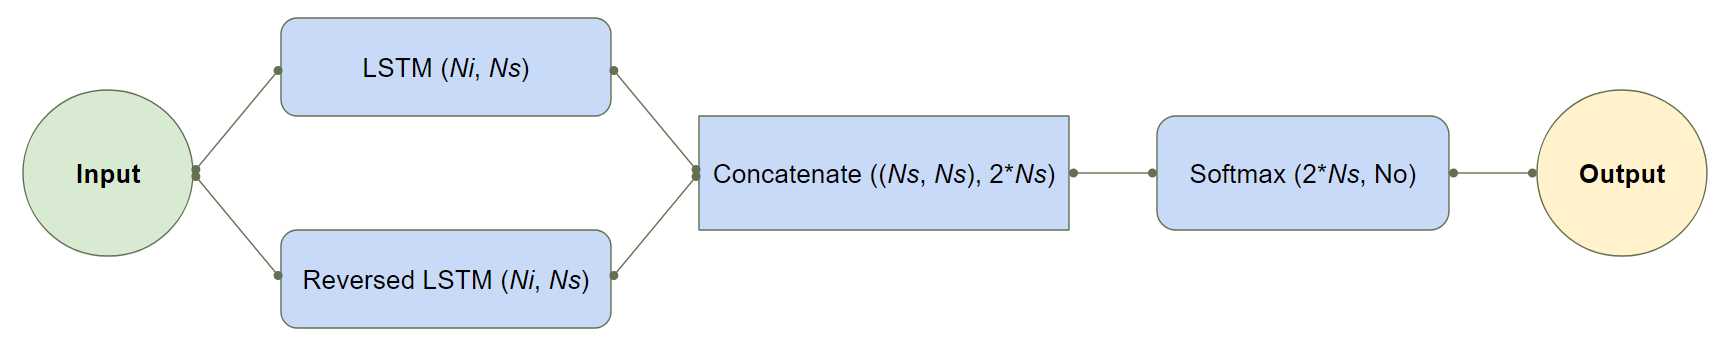
\includegraphics[width=10cm]{img/nn.png}
	\caption{Le réseau utilisé par \texttt{ocropy}}
	\label{nn}
\end{figure}

L'entrée est un \textit{batch} d'images dont la largeur est variable mais la hauteur est fixée à $Ni$. $Ns$ est le nombre de cellules d'états dans le \textit{LSTM}, et également la taille de la sortie de ce réseau. Enfin, $No$ est le nombre de classes. \\
L'entrée est envoyée dans un \textit{LSTM} qui parcourt l'image de gauche à droite et un autre "renversé" qui la parcourt de droite à gauche. Les deux sorties sont ensuite concaténées pour être envoyées dans un layer \textit{Softmax} pour obtenir les classes. \\
La fonction de perte utilisée est la \textit{CTC-loss} (\textit{Connectionist Temporal Classification}) qui est une fonction de perte classiquement utilisée pour les réseaux récurrents. Nous reviendrons dessus plus tard.

\subsection{Utilisation d'ocropy}

Nous avons dans un premier temps téléchargé et installé \texttt{ocropy}.
Le but fut d'abord de comprendre comment l'utiliser.

\subsubsection{Préparation des données}

Afin de nous familiariser avec cet outil, nous avons commencé par binariser et extraire des lignes d'un manuscrit pris sur le site \url{http://www.e-codices.unifr.ch} nous-même.
Ce premier test nous a permis de bien comprendre les premiers enjeux.
En effet, arrivés à l'étape d'annotation des données, nous avons été confrontés à la difficulté que représente la traduction de ces manuscrits.

Par la suite, nous avons abandonné ces données au profit de données annotées nous ayant été mises à disposition par l'ENC.
Parmi ces données, nous avons commencé par travailler sur un manuscrit de la \textit{Chanson d'Otinel} écrit en anglo-normand au XIIIème siècle.
Il est d'une longueur de 46 pages, d'environ 30 lignes chacune. Nous avons pris environ 1300 lignes pour l'entraînement et 100 pour la validation.

\subsubsection{Commandes basiques}

La commande naïve à exécuter pour entraîner un modèle est :

\begin{center}
    \texttt{ocropus-rtrain -o <ModelName> <training-dir>/*/*.bin.png}
\end{center}

On peut également visualiser les étapes avec la commande:

\begin{center}
    \texttt{ocropus-rtrain -o <ModelName> -d 1 <training-dir>/*/*.bin.png}
\end{center}

\noindent A chaque itération, on a un output de la forme suivante : 

\begin{figure}[!h] 
    \center
    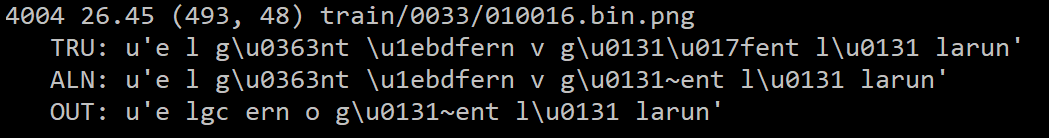
\includegraphics[width=8cm]{img/screen_output.png}
    \caption{Output d'une itération de l'entraînement}
    \label{API}
\end{figure}

Sur la première ligne se trouve d'abord le numéro de l'itération, puis quelques propriétés de l'image étudiée. L'information se contenant dans le lignes suivantes:
\begin{itemize}
    \item \texttt{TRU} est la solution recherchée
    \item \texttt{ALN} est une version alignée de \texttt{TRU}, adaptée à la \textit{CTC-loss}
    \item \texttt{OUT} est le résultat trouvé par le réseau de neurones
\end{itemize}

Afin de lancer la validation d'un modèle et d'avoir le pourcentage d'erreur, on utilise les commandes suivantes :

\begin{center}
    \texttt{ocropus-rpred -m <ModelName> <test-dir>/*/*.bin.png}

    \texttt{ocropus-errs <test-dir>/*/*.gt.txt} permet d'évaluer la précision du modèle.

    \texttt{ocropus-econf <test-dir>/*/*.gt.txt} donne les erreurs les plus fréquentes.
\end{center}

On peut ajouter \texttt{-C2} pour une contextualisation des erreurs.

Sur ce premier entraînement sans préparations, on obtient une erreur de l'ordre de 27\% au bout de 12 000 itérations ce qui est extrêmement mauvais. En effet, l'ensemble des caractères sortant de l'ordinaire ne sont pas reconnus.

\subsubsection{Entraînement avec les caractères spéciaux}

Afin d'intégrer les caractères spéciaux à la résolution, la méthode est de les ajouter à la liste des caractères, stockée dans \texttt{char.py}. C'est ce que nous avons fait, mais cela n'a rien changé. Nous avons compris par la suite que nos modifications effectuées étaient correctes, mais qu'il faut relancer la commande d'installation pour les prendre en compte ...

\begin{center}
    \texttt{sudo python setup.py install}
\end{center}

Ceci nous a permis d'obtenir une première courbe d'erreur satisfaisante.
Le tracé est réalisé en analysant les modèles sauvegardés toutes les 1000 itérations, et en inscrivant les résultats dans des documents \texttt{.txt}.
Un \textit{parsing} avec python permet de récupérer les informations utiles de ceux-ci. 
Le temps nécessaire pour effectuer 1000 itérations est d'environ 11 minutes sur l'ordinateur que nous avons utilisé pour notre installation \texttt{ocropy}.
C'est un portable MSI doté d'une NVIDIA GeForce GTX 1060, le GPU étant le plus important pour entraîner un réseau de neurones.


\subsection{Modification des paramètres d'entraînement}

\subsubsection{Commandes utiles}

Pour modifier l'apprentissage, on peut ajouter une des lignes suivantes à la fin de la commande pour lancer l'entraînement, afin d'en modifier les propriétés.

\texttt{--ntrain <Number>} permet de modifier le nombre d'itérations réalisées dans l'entraînement.
Par défaut il vaut $10^6$, mais en général nous nous arrêtons vers $10^5$ itérations.

\texttt{--savefreq <Number>} permet de dire le nombre d'itérations entre chaque sauvegarde du modèle.
Ceci nous permettra dans la suite de tracer les courbes d'erreur.
Le paramètre par défaut est 1000 et est un bon compromis entre la précision des courbes et le temps passé à tester les modèles.

\texttt{--lrate <Number>} permet de modifier la vitesse d'apprentissage (\textit{learning rate}).
Un de nos premiers objectifs sera de trouver une bonne valeur de ce paramètre.
On rappelle que la \textit{learning rate}, vitesse d'apprentissage, ou vitesse d'entraînement, est un hyper-paramètre qui caractérise le pas dans la descente du gradient stochastique présente dans le réseau de neurone.

\texttt{--hiddensize <Number>} permet de modifier un des paramètres de la taille des matrices de notre réseau de neurones.
Nous nous intéresserons également à son optimisation.

Dans les sous-sections suivantes, nous travaillons avec les données obtenues avec la première normalisation.

\subsubsection{Modification de la taille de cellule}

Le paramètre sur lequel on joue ici est le paramètre définissant le nombre de \textit{hidden states}.
Ce sont les variables que le \textit{LSTM} utilise pour garder une trace du temps.
C'est la partie récurrente du réseau.
L'influence de ce paramètre est présentée figure \ref{err_size}.

\begin{figure}[!h] 
    \center
    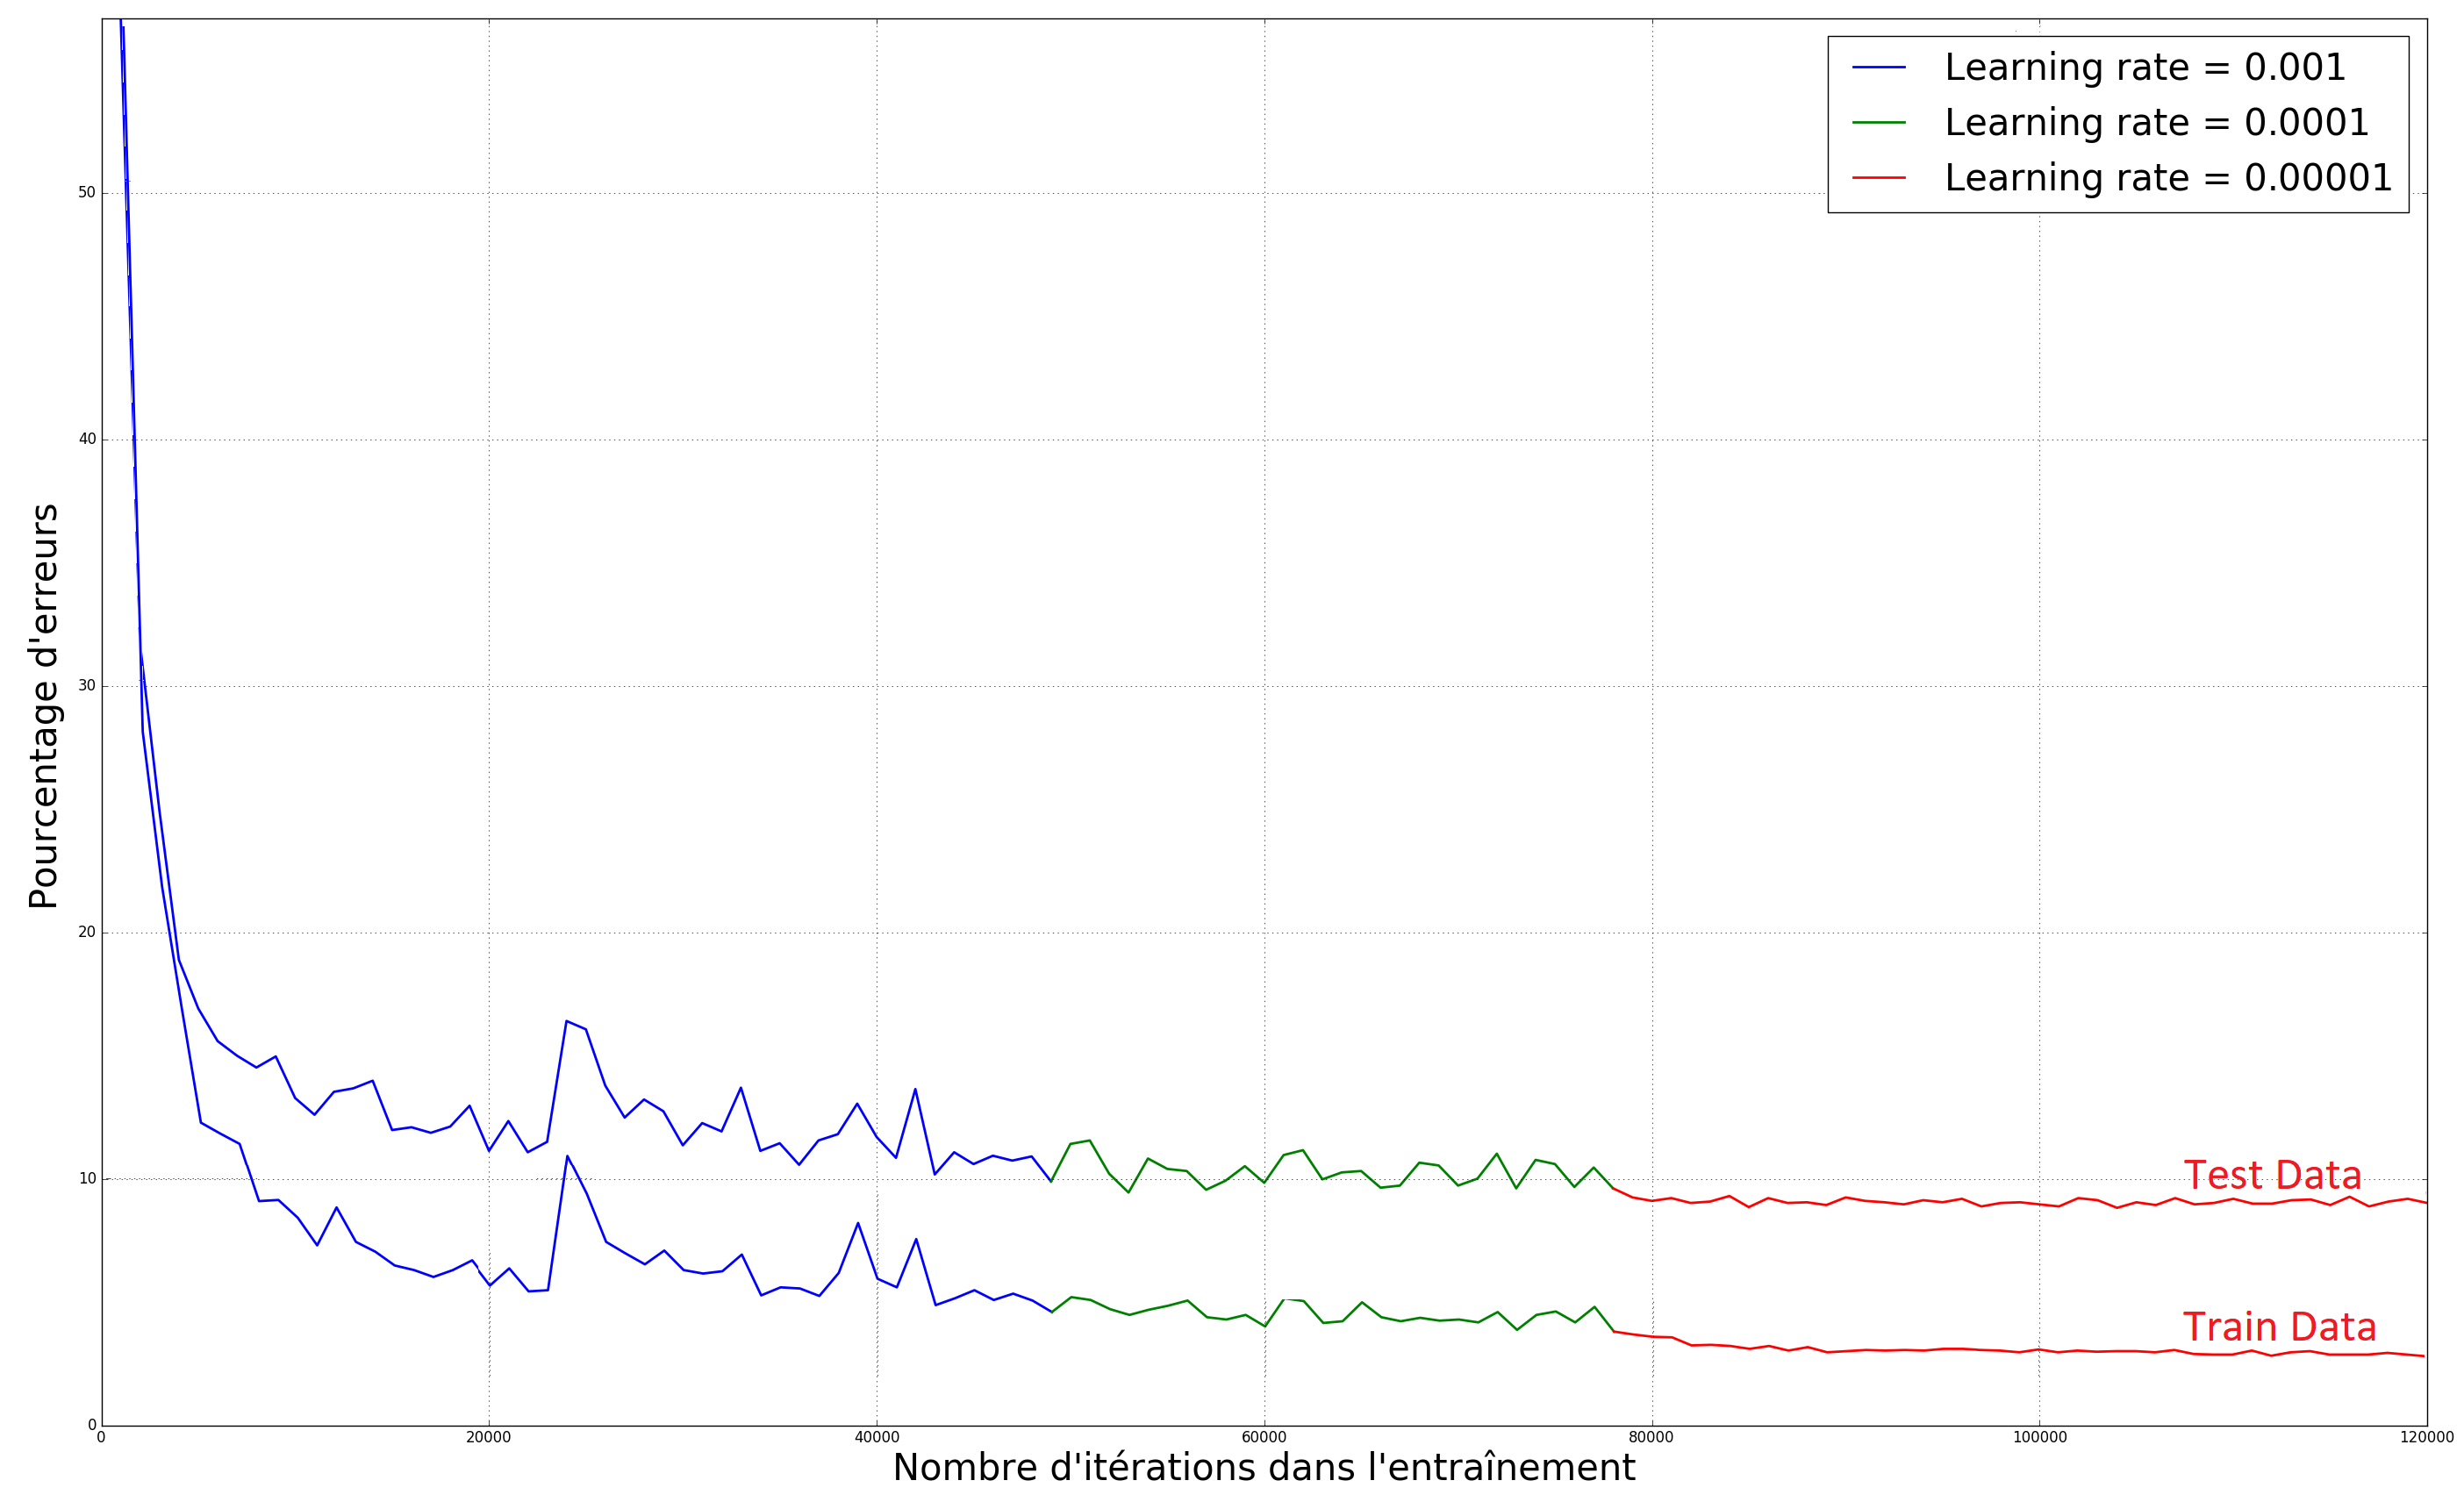
\includegraphics[width=8cm]{img/curve_100.png}
    \caption{Évolution de l'erreur pour \textit{hiddensize} = 100.}
    \label{err_size}
\end{figure}

\begin{figure}[!h] 
	\center
	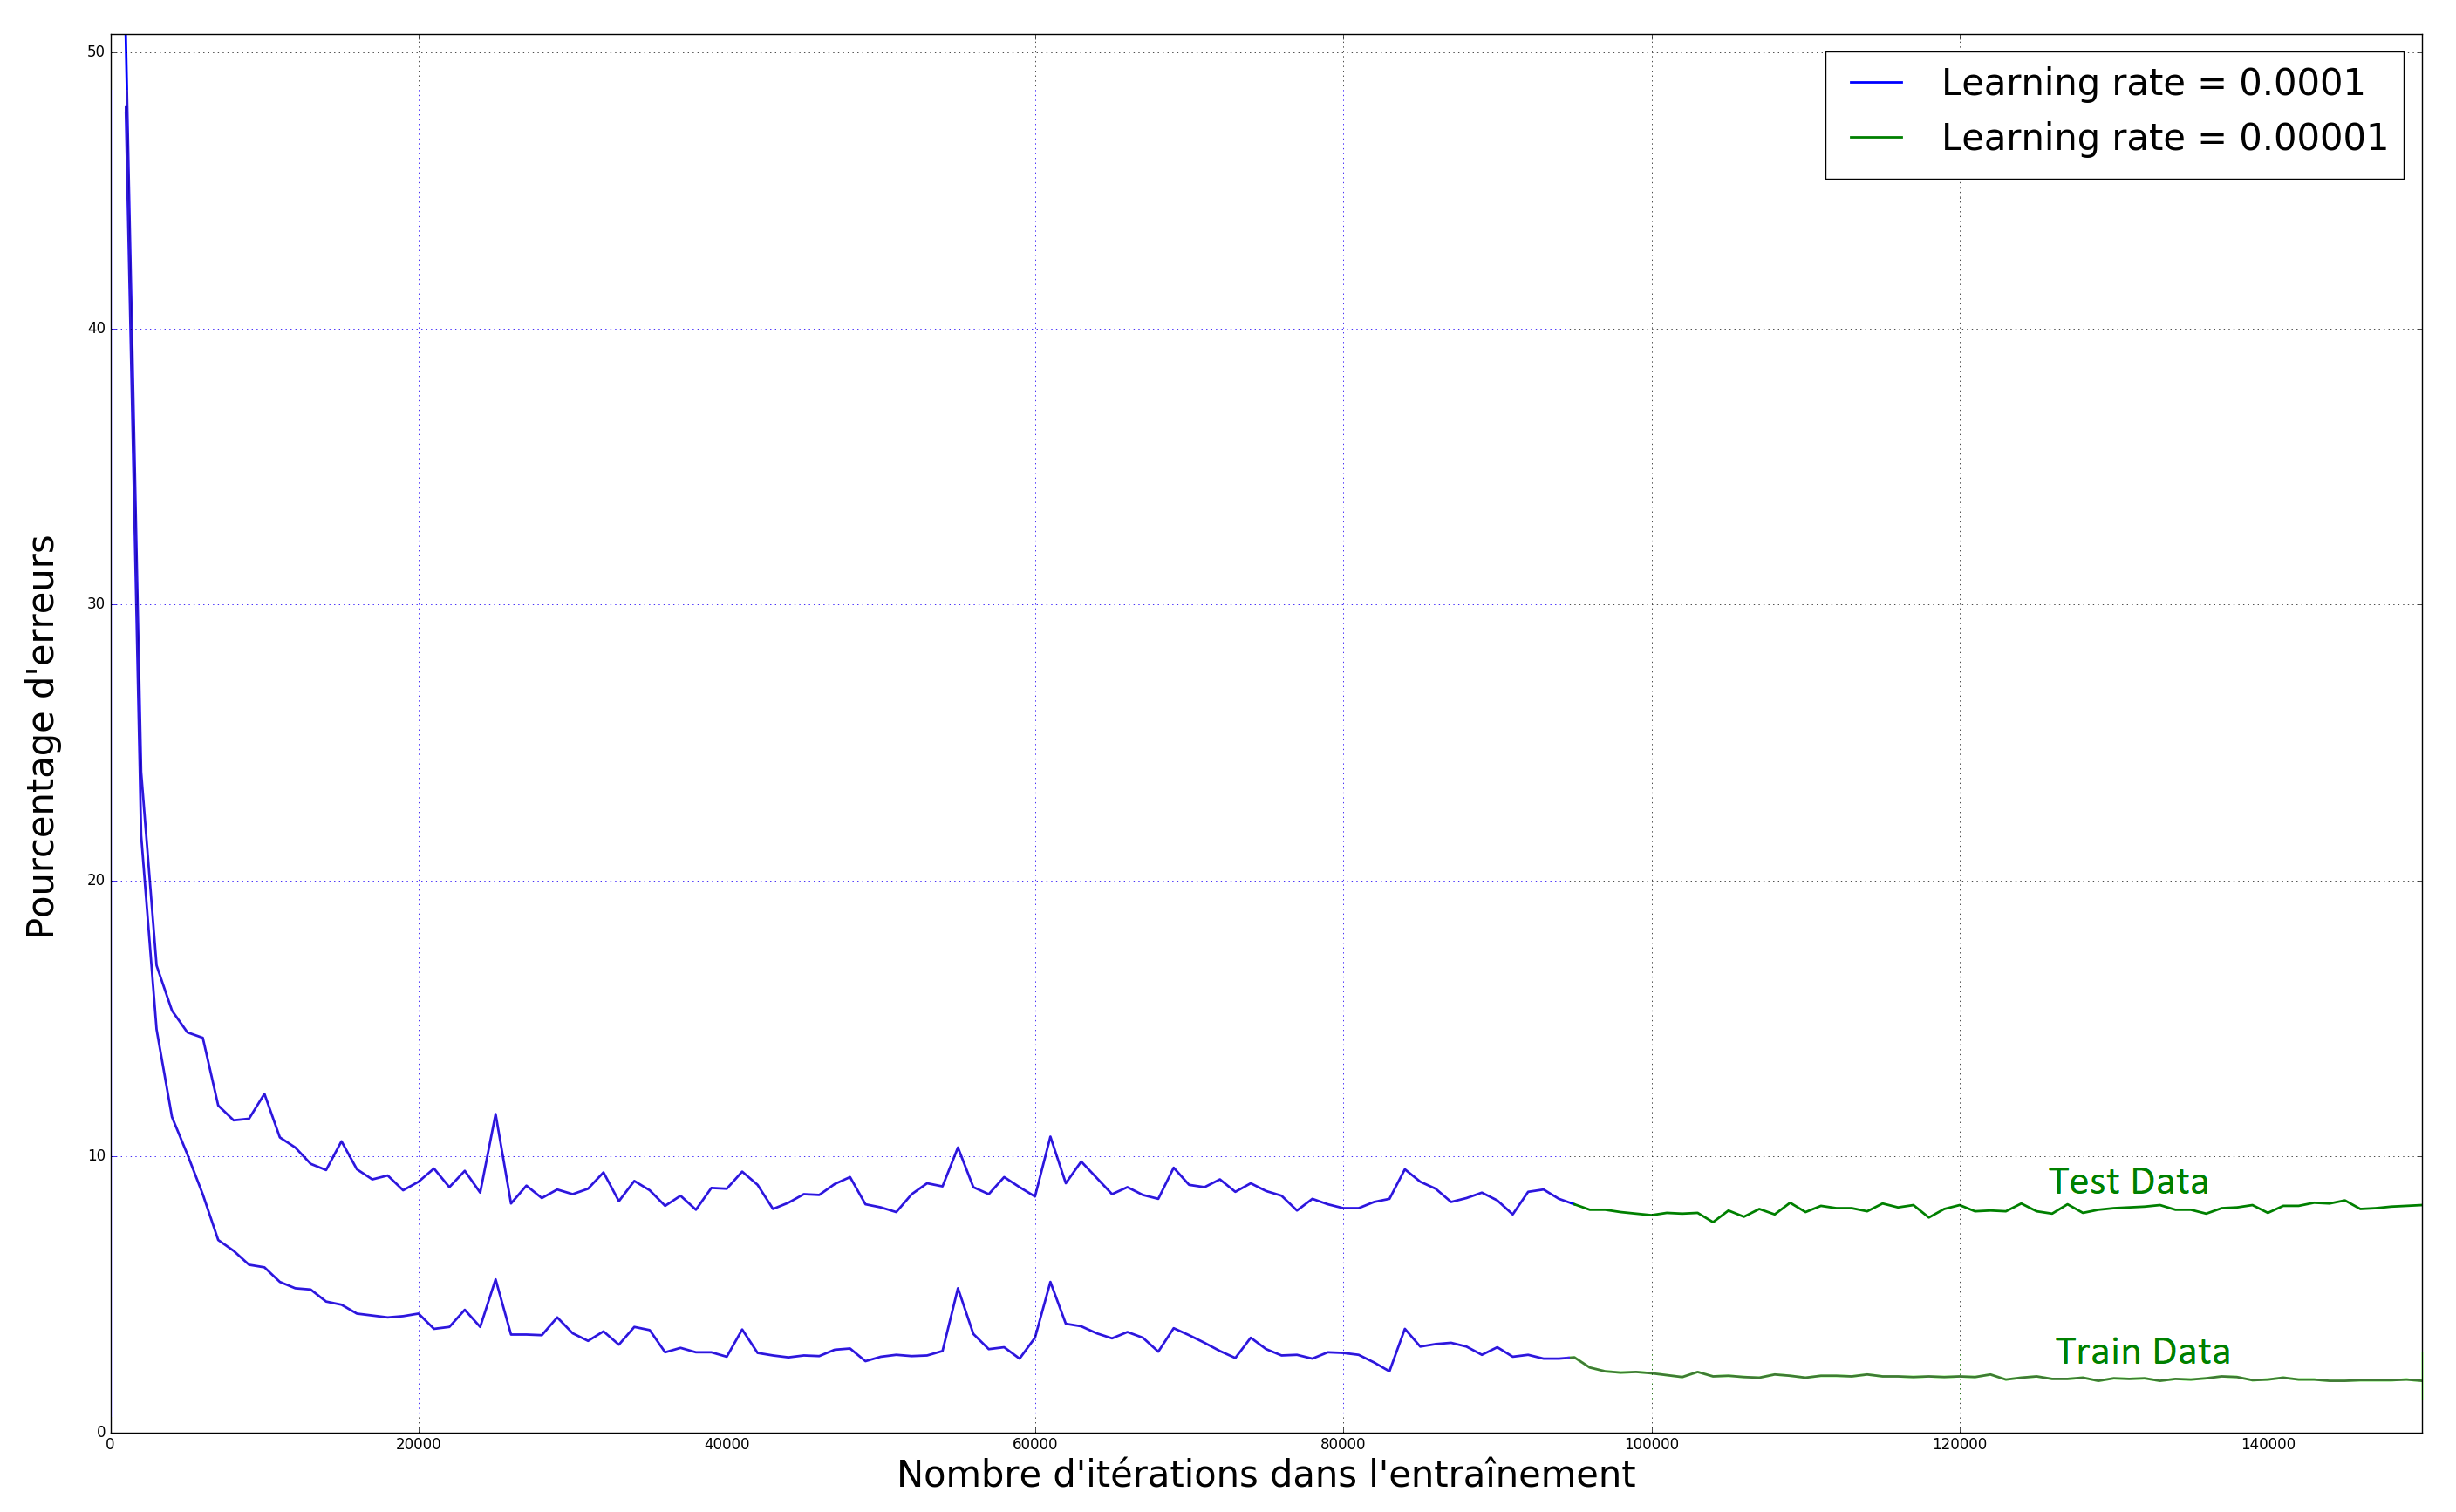
\includegraphics[width=8cm]{img/curve_200.png}
	\caption{Évolution de l'erreur pour \textit{hiddensize} = 200.}
	\label{err_size}
\end{figure}

\begin{figure}[!h] 
	\center
	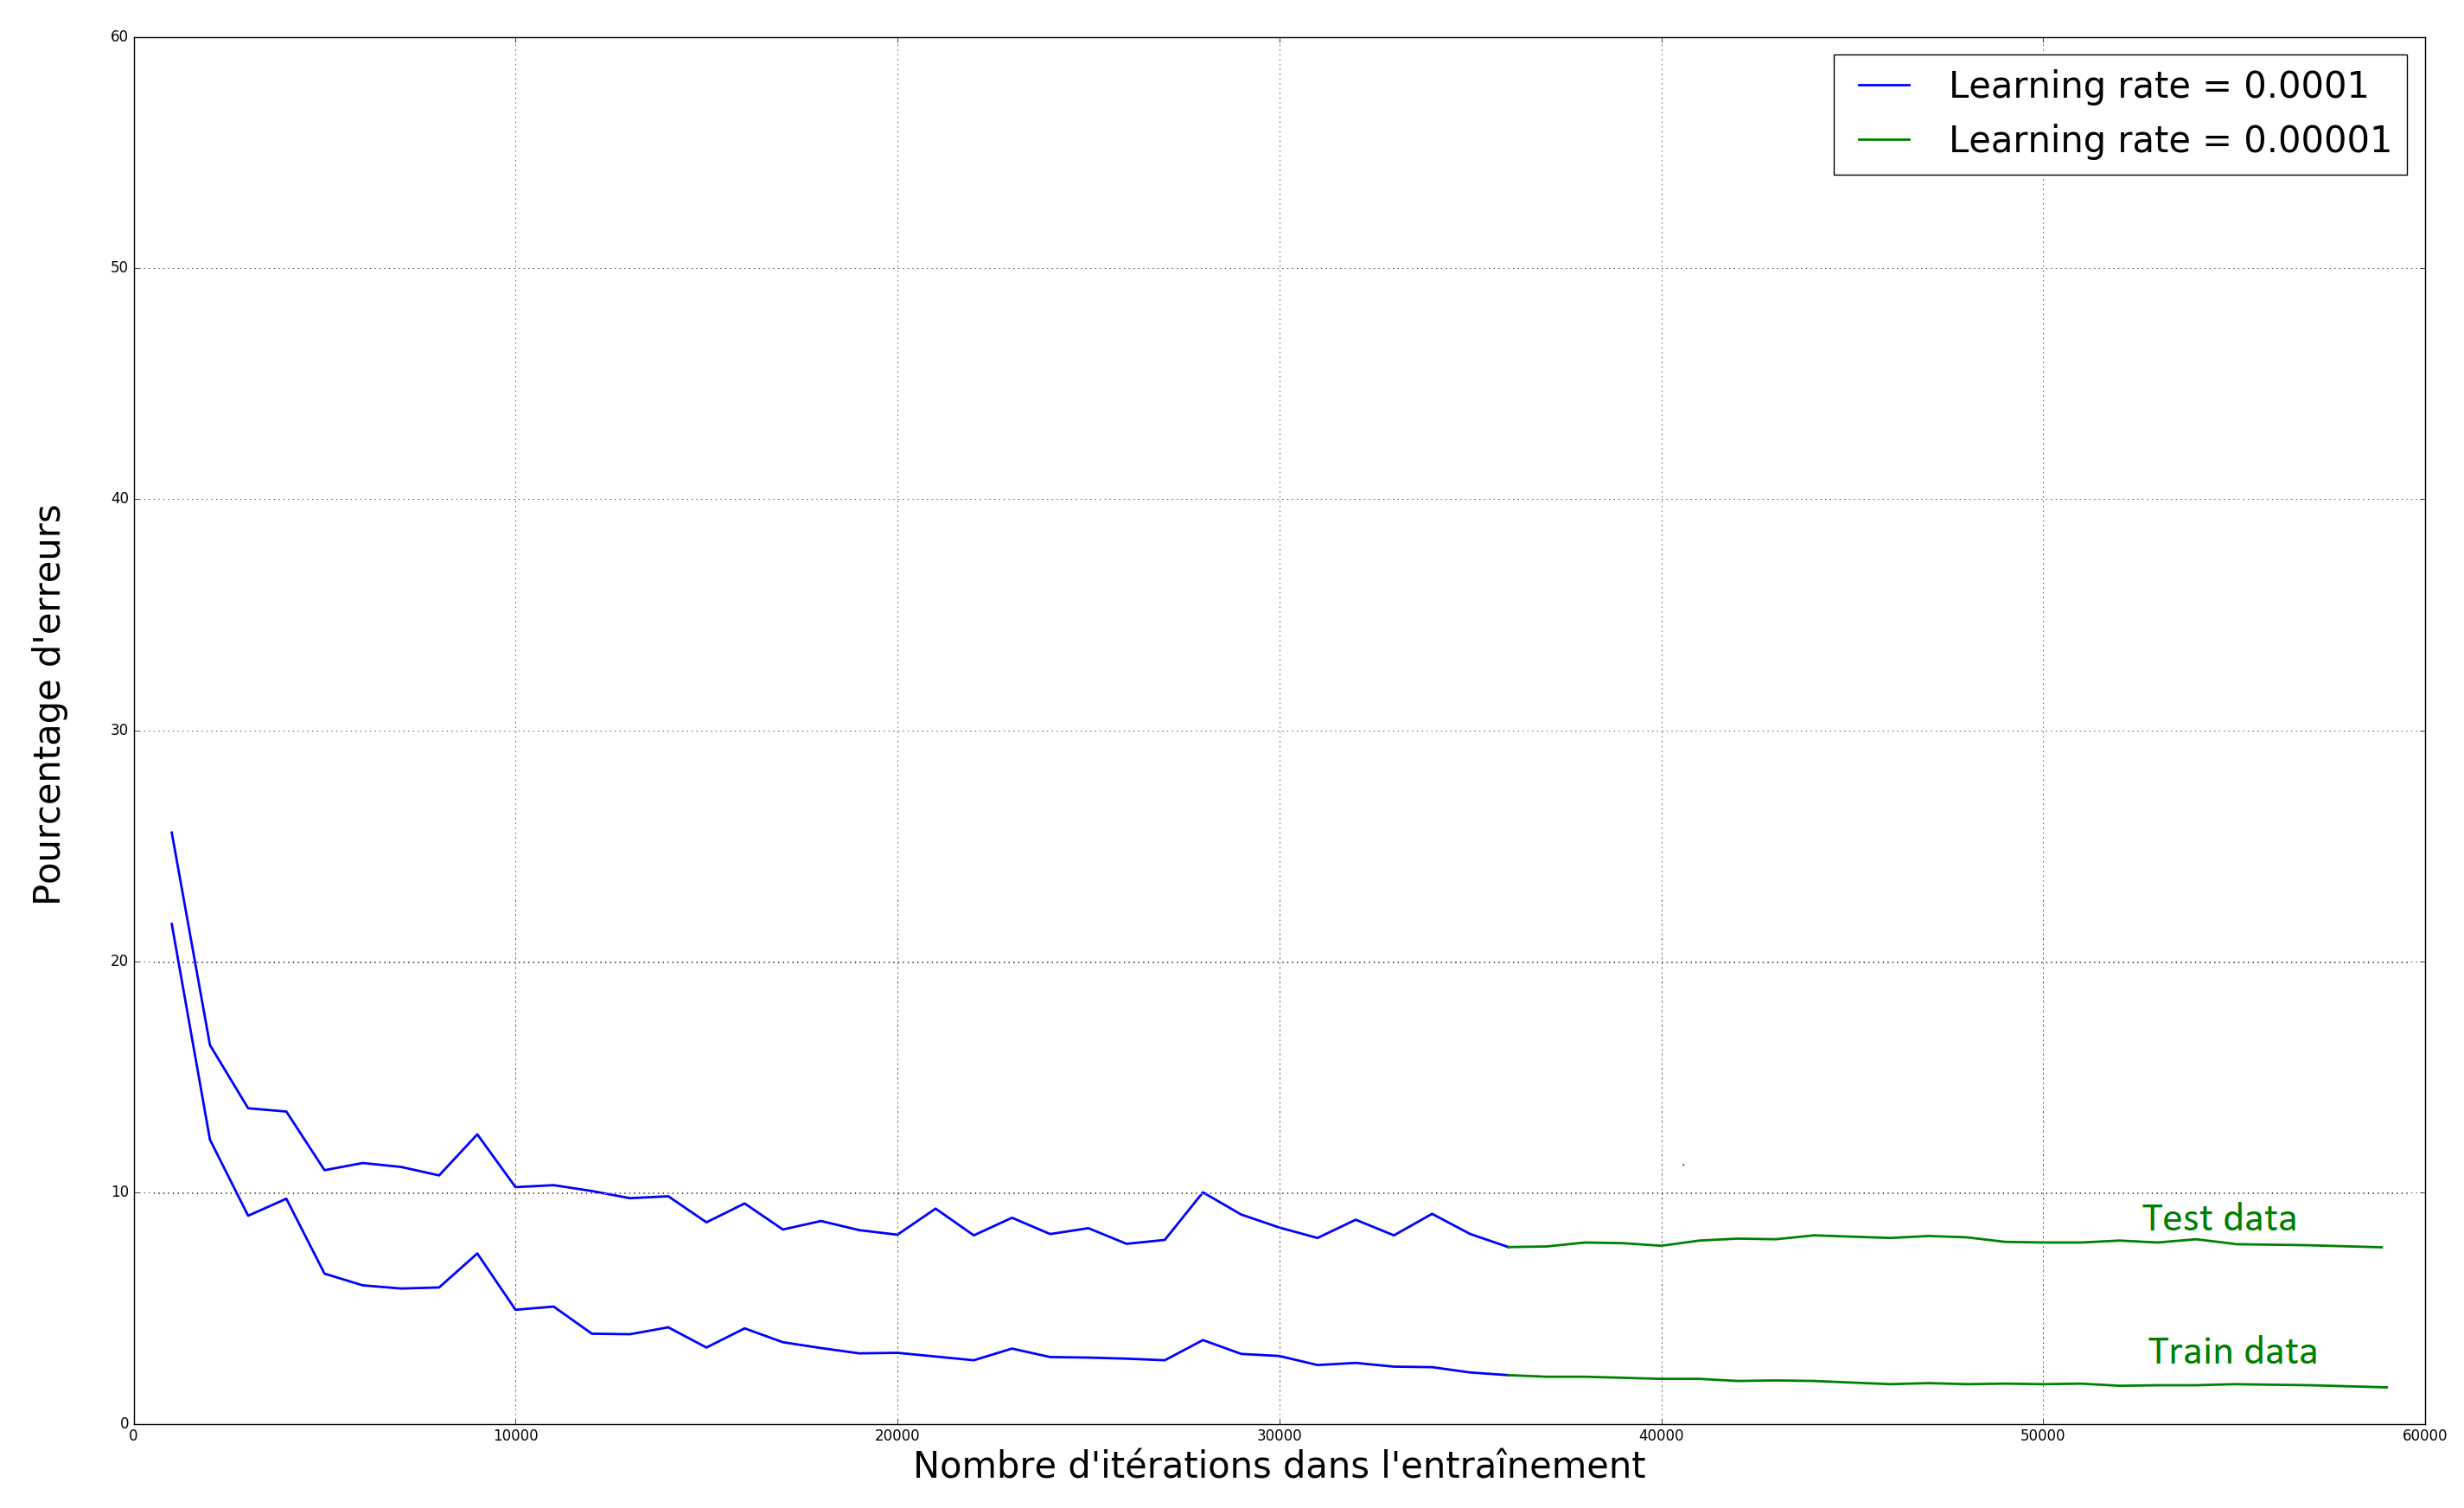
\includegraphics[width=8cm]{img/curve_500.png}
	\caption{Évolution de l'erreur pour \textit{hiddensize} = 500.}
	\label{err_size}
\end{figure}

A priori, plus la taille du réseau est grande, meilleurs sont les résultats. Cependant, on sur-apprend notamment pour le réseau de taille 500. De plus, le temps pour entraîner est multiplié par $1.5$ quand on multiplie par 2 la taille du réseau.

\begin{figure}[!h] 
	\center
	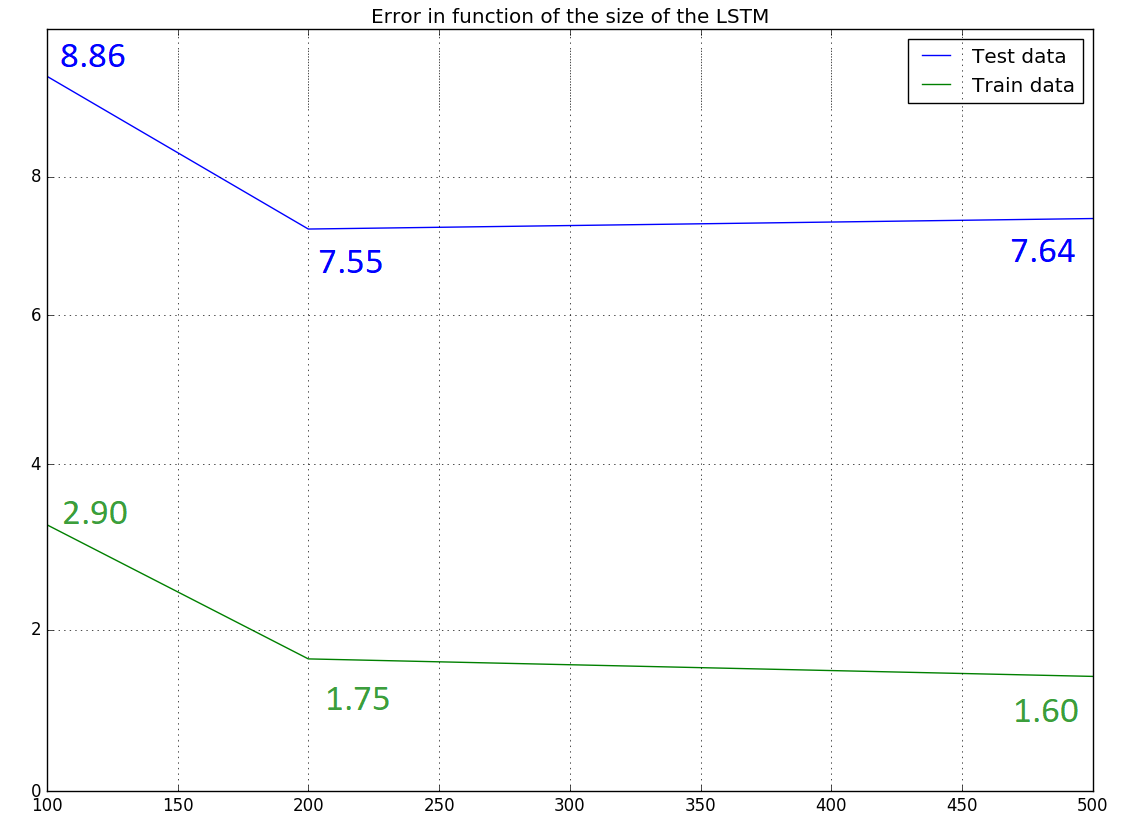
\includegraphics[width=6cm]{img/curves.png}
	\caption{Comparaison des meilleurs modèles obtenus selon les tailles de cellule.}
	\label{err_size}
\end{figure}


\FloatBarrier
\newpage
\newpage

\section{Tesseract}

\subsection{Présentation de Tesseract}

\textbf{Tesseract} est un outil d'OCR, développé par HP en 1985.
Il est depuis devenu Open Source, et est maintenu par Google depuis 2006.
Il est souvent considéré comme l'un des meilleurs moteur d'OCR.

\subsubsection{Utilisation de Tesseract}

Tesseract s'utilise comme ocropy en ligne de commande.
L'utilisation la plus simple est pour lire le texte d'une image dans une langue pour un modèle existant.

\texttt{tesseract imagename|stdin outputbase|stdout}

Google ayant entrainé des modèles dans plus de 50 langues sur des millions de caractères pour des milliers de polices différentes, les résultats sont incroyables.

\subsubsection{Entrainement de Tesseract}

C'est en voulant entrainer Tesseract que nous avons constaté de nombreux défauts.

Dans sa récente version incluant les réseaux LSTM, créer des modèles relève du défi aussi bien technique que psychologique.
La documentation à ce propos est inintelligible pour les personnes n'étant pas initiée aussi bien dans la vision artificielle qu'à l'utilisation avancée des versions précédentes de Tesseract, mais elle est en plus incomplète et indigeste.
Une des raisons à cela serait probablement que l'outil est encore en version alpha, mais aussi que la plupart des personnes autour du projet considèrent que le code en lui-même constitue un élément suffisant pour pouvoir savoir entrainer des modèles soi-même.

Tesseract est donc un puissant outil pour la reconnaissance de caractères dans des langues ayant déjà été entrainées, mais dans le cadre de notre problème il ne semble pas adapté.
En effet, il nous faudrait un outil adaptable à de nombreuses langues et écritures.

\chapter{Création d'une solution OCR}

\section{Principe du réseau de neurone appliqué à l'OCR}

Supposons que l'on traite une image $I(x, y)_{x \in [0, W[,\ y \in [0, H[}$.
Quand on y lit le texte, on balaie l'image de gauche à droite, et on détermine les lettres puis les mots étant donné ce que l'on voit à l'instant combiné à ce que l'on a vu précédemment.
On peut donc considérer la lecture du texte sur l'image comme un procédé séquentiel, où l'on a une entrée $X_t = \left(I(t, y)\right)_{y\in [0, H[}$.oChaque $X_t$ est donc une colonne de 1 pixel de large et $H$ pixels de haut.

On peut alors utiliser un réseau neuronal récurent (\emph{RNN}).
Le principe d'une couche de neurone récurent est de traîter la séquence étape par étape, en gardant en mémoire un \emph{état} $h_t$.
En combinant l'arrivée de donnée $X_t$ et l'état $h_t$, le RNN va pouvoir capter des patterns dans la séquence et ressortir un output $Y_t$ représentatif des features à cet instant $t$.

En repassant cet output $Y_t$ dans un classifieur, on peut alors déterminer pour chaque colonne de pixel sa probabilité de représenter un caractère.

En pratique, on utilisera la même architecture que le réseau d'ocropy avec :

\begin{itemize}
	\item les données en entrée
	\item un RNN
		\item un LSTM forward
		\item un LSTM backward
	\item un merge des deux sorties
	\item un réseau dense
	\item un softmax
\end{itemize}

\section{La CTC loss}

Brièvement, la CTC Loss est une solution technique au problème suivant :
étant donné qu'une image à traiter peut posséder entre 800 et 2000 colonnes de pixels, comment labeliser l'image ?

Une approche naïve serait de labeliser pour chaque colonne la lettre qu'elle est censé représenter.
D'une part le problème devient trop contraignant, d'autre part ce type de précision ne nous intéresse pas.
En effet, si le réseau est capable de détecter une lettre uniquement par son début, uniquement par son milieu, ou uniquement par sa fin, ce fonctionnent complique inutilement le problème d'apprentissage.
D'autre part, on ne peut comparer naïvement une séquence de 2000 sorties du réseau et un label représentant le texte qui serait ayant une taille aux alentours de 30 ou 40.

La CTC répond à ces problématiques.

\textit{
Nous avons présentée ses spécificités technique à l'oral.
Si nécessaire, nous pouvons ré-expliquer ici son fonctionnement.
}

\section{Développement avec Keras}

Keras est un wrapper pour faire des architectures de Deep Learning, fonctionnant avec TensorFlow, Theano et CNTK.
Nous avons choisi ce module car sa modularité avec plusieurs \emph{backends} le rend très portable, ce qui est important si l'on veut développer une solution elle-même portable et utilisable par une majorité de personnes.

Des expérimentations sont disponibles dans le dossier \textit{neuralnetworks} du repository du projet.

Nous avons ensuite implémenter une solution d'OCR. Le github est publique :

https://github.com/GuillaumeDesforges/simple-ocr

Une des difficulté a été d'utiliser les fonctions relative à la CTC (la loss et le décodage).
Leur utilisation n'est en effet pas direct comme les autres fonctions et couches, et elles sont peu documentées.
Une compréhension des calculs réalisés (création des graphes fonctionnels par exemple) ont été nécessaires pour arriver à mettre en oeuvre ces fonctions.

Dans ce repository, la partie relative à la GUI est dans le dossier \textit{app} et la partie relative à l'entraînement des réseaux est dans le dossier \textit{engine}.

\appendix
\end{document}
